\documentclass[8pt]{beamer}
\usetheme{default} % Very simple theme
\usecolortheme{dove} % Minimalist grayscale colors
\setbeamertemplate{navigation symbols}{} % Remove navigation bar

% Define brand-like colors
\definecolor{myblue}{RGB}{0, 102, 204}    % Blue for standard blocks
\definecolor{mygreen}{RGB}{0, 153, 0}     % Green for example blocks
\definecolor{myred}{RGB}{204, 0, 0}       % Red for alert blocks
\definecolor{myorange}{RGB}{255, 128, 0} % For \emph

% Accent color for titles, bullets, etc.
\setbeamercolor{structure}{fg=myblue}

% Block colors
\setbeamercolor{block title}{bg=myblue, fg=white}
\setbeamercolor{block body}{bg=blue!5, fg=black}

\setbeamercolor{exampleblock title}{bg=mygreen, fg=white}
\setbeamercolor{exampleblock body}{bg=green!5, fg=black}

\setbeamercolor{alertblock title}{bg=myred, fg=white}
\setbeamercolor{alertblock body}{bg=red!5, fg=black}
\setbeamercolor{alerted text}{fg=myred}

% Optional: color for \example text
\setbeamercolor{example text}{fg=mygreen}

% Custom emph (orange text instead of italic)
\let\oldemph\emph
\renewcommand{\emph}[1]{\textcolor{myorange}{#1}}
\newcommand{\ve}[1]{\boldsymbol{#1}}

\usepackage{graphicx} % Package for images
\usepackage{amsmath} % Package for images
\graphicspath{{figs/}} % Path to your figures directory
\usepackage{array}  % For better column spacing
\usepackage{caption} % Required for \captionof
%\usepackage{enumitem}

% Title Information
\title{STOCHASTIC METHODS IN WATER RESOURCES}
\vspace{25pt}
\subtitle{Unit 5: Geostatistics \\ Lecture 18: Other kriging and geostatistical simulation}
\author{Luis Alejandro Morales, Ph.D.}
\institute{Universidad Nacional de Colombia \\ Department of Civil and Agriculture Engineering} %// }
%\date{\today}

\begin{document}

% Title Slide
\begin{frame}
    \titlepage
\end{frame}

%-------
% From Bierkens
\section{Log-normal kriging}
 \begin{frame}{Log-normal kriging}
     \begin{block}{Generalities}
    \end{block}
    \begin{itemize}
        \item Many geophysical variables, such as \emph{hydraulic conductivity} and \emph{pollutant concentration}, are approximately \emph{log-normal distributed}.
        \item A frequently used \emph{random space function} model to decribe these variables is the \emph{multivariate log-normal distribution}.
        \item If $Z(\mathbf{x})$ is \emph{multivariate log-normal distributed}, the natural logarithm $Y(\mathbf{x})=\ln(Z(\mathbf{x}))$ is \emph{multivariate normal distributed}. \alert{Log-normal kriging} then consists of the following steps:
            \begin{enumerate}
                \item Transform the observations $z(\mathbf{x}_i)$ by taking their logarithms $y(\mathbf{x}_i) = \ln(z(\mathbf{x}_i))$.
                \item Estimate the \emph{semivariogram} $\hat{\gamma}_Y (\mathbf{h})$ from the log-transformed data $y(\mathbf{x}_i)$ and fit a permissible model (note: that mean $m_Y$ must be determined and assumed known if \emph{simple kriging} is used). u                
                \item Using the \emph{semivariogram} $\hat{\gamma}_Y (\mathbf{h})$, the data $y(\mathbf{x}_i)$ (and the mean $m_Y$ in case of \emph{simple kriging}), the kriging equations are solved to obtain at every non-observed location $\mathbf{x}_0$ the prediction $\hat{Y}_{SK} (\mathbf{x}_0)$ and prediction error variance $\sigma_{YSK}^2 (\mathbf{x}_0)$ in cased of \emph{simple kriging} or $\hat{Y}_{OK} (\mathbf{x}_0)$, $\hat{Y}_{YOK} (\mathbf{x}_0)$ in case of \emph{ordinary kriging}.
                \item An unbiased prediction of $Z(\mathbf{x}_0)$ is obtained by the following backtransforms footnote:
                    \begin{itemize}
                        \item for \emph{simple kriging}:
            \begin{equation}
                \hat{Z}(\mathbf{x}_0) = e^{\hat{Y}_{SK} (\mathbf{x}_0) + \frac{1}{2}\sigma_{YSK}^2}
                \label{e732}
            \end{equation}
                        \item for \emph{ordinary kriging}:
            \begin{equation}
                \hat{Z}(\mathbf{x}_0) = e^{\hat{Y}_{OK} (\mathbf{x}_0) + \frac{1}{2}\sigma_{YOK}^2 - \nu_Y}
                \label{e733}
            \end{equation}
            where $\nu_Y$ is the \emph{lagrange multiplier} used in the \emph{ordinary kriging} system.

                    \end{itemize}
            \end{enumerate}
    \end{itemize}
\end{frame}

 \begin{frame}{Log-normal kriging}
     \begin{block}{Generalities}
    \end{block}
%    \begin{itemize}
\begin{enumerate}
    \setcounter{enumi}{4} % continues from item 3
    \item If $Y(\mathbf{x})$ is \emph{multivariate Gaussian} distributed and \emph{stationary}, the \emph{conditional cumulative probability distribution function} can be calculated from the \emph{simple kriging} prediction $\hat{y}_{SK}(\mathbf{x}_0)$ and prediction \emph{variance} as:
            \begin{equation}
                F_{z|z_1,\cdots,z_n} (z; \mathbf{x}_0 | z(\mathbf{x}_i), i=1,\cdots,n) = \frac{1}{\sqrt{2\pi \sigma_{YSK}^2 (\mathbf{x}_0)}} \int_{-\infty}^z e^{\frac{-\left[\ln(z)-\hat{y}_{SK}(\mathbf{x}_0) \right]^2}{\sigma_{YSK}^2 (\mathbf{x}_0)}} dz
                \label{e734}
            \end{equation}
            An additional reason why in many geostatistical studies the observations are \emph{log-transformed} before kriging is that the \emph{semivariogram} of log-transforms can be better estimated (shows less noise) because of the imposed \emph{variance} reduction.
\end{enumerate}
%\end{itemize}
\end{frame}

%-------
% From Bierkens
\section{Kriging normal-score transforms}
 \begin{frame}{Kriging normal-score transforms}
     \begin{block}{Generalities}
    \end{block}
    An even more general \emph{transformation} is the \alert{normal-score transform} using the \emph{histogram}. Through this transform, it is possible to \emph{transform} any set of observations to \emph{univariate Gaussian distributed variables}, regardless of the distribution of these observations. A \emph{normal score-transform} proceeds as follows:
    \begin{enumerate} 
        \item The $n$ observations are \emph{ranked} in ascending order:
            \[
                z(\mathbf{x}_i)^{(1)} \leq z(\mathbf{x}_j)^{(2)} \leq \cdots \leq z(\mathbf{x}_k)^{(r)} \leq \cdots \leq z(\mathbf{x}_l)^{(n)}
            \]
            where $r=1,\cdots,n$ are the \emph{ranks} of the observations.
        \item The \emph{cumulative probability} associated with observation $z(\mathbf{x}_k)$ with rank $r$ is estimated as:
            \begin{equation}
                \hat{F}(z_k) = \frac{r(z_k)}{n+1}
                \label{e735}
            \end{equation}
            or in case of \emph{declustering} 
            \begin{equation}
                \hat{F}(z_k) = \sum_{i=1}^{r(z_k)} w_{r(z_k)}
                \label{e736}
            \end{equation}
        \item The associated \emph{normal score transform} is given by the $\hat{p}_r$-quantile of the \emph{standard normal distribution}:
            \begin{equation}
                y_{ns}(z_k (\mathbf{x}_k)) = N^{-1} \left[\hat{F}(z_k (\mathbf{x}_k)) \right]
                \label{e737}
            \end{equation}
            where $N(z)$ is the \emph{standard Gaussian cumulative distribution function} and $N^{-1}(p)$ its \emph{inverse}.
    \end{enumerate} 
\end{frame}

 \begin{frame}{Kriging normal-score transforms}
     \begin{block}{Generalities}
    \end{block}
    The figure below shows graphically how the \emph{normal-score transform} works. The left figure shows the estimated \emph{cumulative distribution} of the original (non-transformed) data and the right figure the \emph{standard Gaussian cumulative distribution}. The dashed lines show how the observed values $z_k$ are transformed into the \emph{normal-score transform} $y_{ns}(z_k)$.
        \begin{center}
            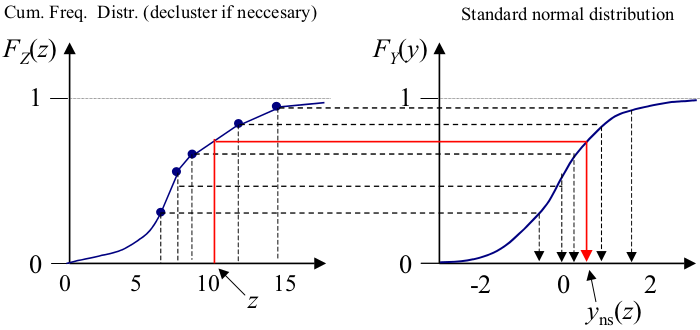
\includegraphics[width=\linewidth]{fiBi714.png}  % from Bierk
        \end{center}

\end{frame}

 \begin{frame}{Kriging normal-score transforms}
     \begin{block}{Generalities}
    \end{block}
            \vspace{-5pt}
    If we assume that the \emph{normal-score transforms} are \emph{stationary} and \emph{multivariate Gaussian distributed},  the local pdfs can be obtained through \emph{simple kriging} as follows:
    \begin{enumerate}
        \item Perform a \emph{normal score transform} of the observations such as decribed above.
        \item Estimate the \emph{semivariogram} of the \emph{normal-score transformed data} $y_{ns}(\mathbf{x}_k) = y_{ns}(z(\mathbf{x}_k))$ and fit a permissible semivariogram model $\gamma_Y (\mathbf{h})$. By definition, the mean value of the \emph{transformed random space function} $Y_{ns} (\mathbf{x}_0)$ is zero.
        \item Use the fitted \emph{semivariogram model} and the \emph{normal-score transforms} $y_{ns} (\mathbf{x}_k)$ in the \emph{simple kriging} equations (with $m_Y =0$) to obtain the \emph{prediction} $\hat{Y}_{SK} (\mathbf{x}_0)$ and the associated \emph{prediction error variance} $\sigma_{YSK}^2 (\mathbf{x}_0)$.
        \item The local \emph{cdf} is then given by
            \vspace{-5pt}
            \begin{equation}
                \begin{aligned}
                    &F_{z|z_1,\cdots,z_n} (z; \mathbf{x}_0 | z(\mathbf{x}_i), i=1,\cdots,n) \\
                    &= Pr\left[G\left(\hat{y}_{SK}(\mathbf{x}_0), \sigma_{YSK} (\mathbf{x}_0) \right) \leq y_{ns} (z) \right]\\
                    &= \frac{1}{\sqrt{2\pi \sigma_{YSK}^2 (\mathbf{x}_0)}} \int_{-\infty}^z e^{\frac{-\left[y_{ns}(z)-\hat{y}_{SK}(\mathbf{x}_0) \right]^2}{\sigma_{YSK}^2 (\mathbf{x}_0)}} dz
                \end{aligned}
                \label{e738}
            \end{equation}
            where $y_{ns} (z)$ is the \emph{normal-score transform} of the value $z$ and $G(\mu, \sigma)$ a \emph{Gaussian variate} with \emph{mean} $\mu$ and \emph{variance} $\sigma$.
    \end{enumerate}
    This is also shown graphically in figure above. Suppose we want to known for the non-observed location the probability that $Z(\mathbf{x}_0) \leq z$. We first obtain through the transformation the value of $y_{ns}(z)$. From the \emph{simple kriging} of transformed data we have at $\mathbf{x}_0 : \hat{y}_{SK}(\mathbf{x}_0)$ and $\sigma_{YSK}^2 (\mathbf{x}_0)$. Finally, we evaluate $Pr\left[G\left(\hat{y}_{SK}(\mathbf{x}_0), \sigma_{YSK}(\mathbf{x}_0)\right) \leq y_{ns}(z)\right]$ (see equation~\ref{e738}) to obtain the probability.
\end{frame}

 \begin{frame}{Kriging normal-score transforms}
     \begin{block}{Generalities}
    \end{block}
    \begin{itemize}
        \item To calculate the \emph{normal-score transform} of any given value $z$ (which is not necessarily equal to the value of one of the observations), the resolution of the estimated \emph{cdf} $\hat{F}(z)$ must be increased.
        \item Usually, a \emph{linear interpolation} is used to estimate the values of $\hat{F}(z)$ between two observations (see figure above). Of course, most critical is the \emph{extrapolation} that must be performed to obtain the \emph{lower} and \emph{upper} \emph{tails} of $\hat{F}(z)$.
        \item For instance, if the \emph{upper tail} of $\hat{F}(z)$ rises too quickly to 1, the probability of high values of $z$ (e.g. a \emph{pollutant in groundwater}) may be underestimated.
        \item Usually a \emph{power model} is used to \emph{extrapolate} the \emph{lower tail} and a \emph{hyperbolic model} to \emph{extrapolate} the \emph{upper tail}.
    \end{itemize}
\end{frame}
 \begin{frame}{Kriging normal-score transforms}
     \begin{block}{Generalities}
    \end{block}
    The figure below shows the \emph{histogram} and the \emph{semivariogram} of of the \emph{normal score transforms}. It can be seen that \emph{semivariogram} is less noisy than that of the \emph{non-transformed data}, because transformation decreases the effect of the very large values.
        \begin{center}
            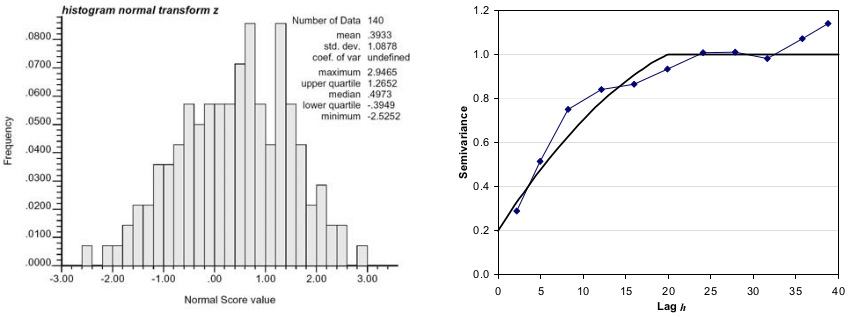
\includegraphics[width=\linewidth]{fiBi715.png}  % from Bierk
        \end{center}
\end{frame}

\begin{frame}{Geostatistical simulation}
     \begin{block}{Generalities}
    \end{block}
    \begin{itemize}
        \item The third field of application of \emph{geostatistics} is simulating realisations of the \emph{conditional random function} $Z(\mathbf{x} | z(\mathbf{x}_i), i=1,\cdots,n$.
        \item The aim of \emph{geostatistical simulation} is to generate in the individual conditional realisations. There are two important reasons why sometimes individual realisations of the conditional \emph{random spatial function} are preferred over the interpolated map that is provided by \emph{kriging}:
            \begin{enumerate}
                \item \emph{kriging} provides a so called \emph{best linear prediction} (it produces values that minimize the \emph{variance of the prediction error}: $var[\hat{Z}(\mathbf{x}_0)-Z(\mathbf{x}_0)]$, but the resulting maps are much smoother than reality.The individual realisations are very noisy and rugged while the \emph{kriging prediction} produces a smoothly varying surface. The \emph{noisy realisations} have a \emph{semivariogram} that resembles that of the data, so one can say that the real variation of the property considered is much more like the realisations than the \emph{kriging map}.
                \item \emph{multiple realisations} as input for a model can be used for \emph{uncertainty analysis} and \emph{ensemble prediction}. We only have limited information about reality and we therefore represent our uncertainty about reality with a random function. Returning to the example of \emph{hydraulic conductivity}, if we are uncertain about the \emph{parameters} of a \emph{groundwater model}, we also want to know what the uncertainty is about the model output (heads, fluxes). So instead of analysing a single input of \emph{hydraulic conductivity}, a large number of conditional realisations of \emph{hydraulic conductivity} (say 1000) are used as model input. The \emph{variance} of the output realisations is a measure of our \emph{uncertainty} about the output (e.g. \emph{hydraulic heads}) that is caused by our \emph{uncertainty} (lack of perfect knowledge) about the \emph{model parameters} (e.g. \emph{hydraulic conductivity}).
            \end{enumerate}
    \end{itemize}
\end{frame}
 \begin{frame}{Geostatistical simulation}
     \begin{block}{Generalities}
    \end{block}
    The figure is a schematic representation of \alert{Monte Carlo simulation} applied for \emph{uncertainty analysis} of \emph{hydraulic conductivity} in \emph{groundwater modelling}. \emph{Hydraulic conductivity} is spatially varying and sampled at a limited number of locations. \emph{Hydraulic conductivity} is modelled as a \emph{random space function}. Using the observations statistics are estimated that characterise this function (\emph{histogram}, \emph{semivariogram}). Next $M$ realisations of this \emph{random function} are simulated and used in the \emph{groundwater model}. This yields $M$ realisations of \emph{groundwater model} output (e.g. \emph{head fields}). From these realisations it is possible to obtain for a given location (e.g. $\mathbf{x}_0$ ) the \emph{probability density function} of the output variables (e.g. \emph{head}, \emph{concentration}).
        \begin{center}
            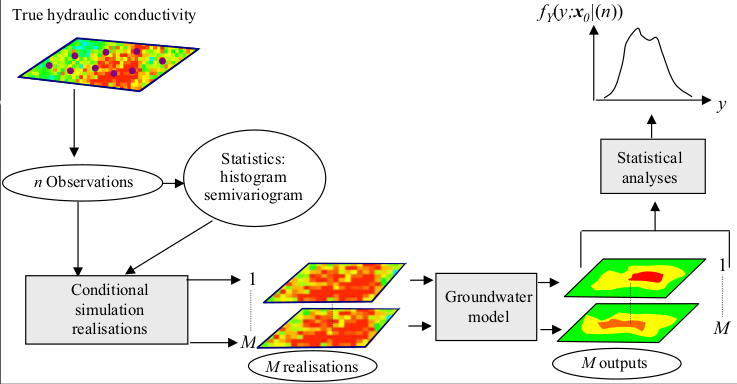
\includegraphics[width=0.85\linewidth]{fiBi717.png}  % from Bierk
        \end{center}

\end{frame}

  \begin{frame}{Geostatistical simulation}
     \begin{block}{Generalities}
    \end{block}
    For the generation of multiple realisations (\emph{Monte Carlo simulations}) of the \emph{conditional random space function}, commonly referred to as (conditional) \emph{geostatistical simulation}. There are quite a few methods for \emph{simulating realisations} of \emph{MultiGaussian random space functions}. The most commonly used are \alert{LU-decomposition}, the \alert{turning band method} and \alert{Sequential Gaussian simulation}, while there are even more methods for \emph{simulating non-Gaussian random functions}. The \emph{most flexible simulation algorithm} and mostly used nowadays is \emph{sequential simulation}. \emph{Sequential Gaussian simulation (sGs)} will be treated here briefly. \emph{Conditional simulation} with \emph{sGs} needs the \emph{mean} $\mu_Z$ and the \emph{semivariogram} of the \emph{random space function} $\gamma_Z(h)$ and proceeds as follows.
    \begin{enumerate}
        \item The \emph{area} is divided into a finite number of grid points $N$ (location indices $\mathbf{x}_1$, $\mathbf{x}_2$,$\cdots$, $\mathbf{x}_N$) at which values of the conditional realisations are to be simulated. The grid points are visited in a random order.
        \item For the first grid point $\mathbf{x}_1$ a \emph{simple kriging} is performed from the given data $z(\mathbf{s}_1),\cdots,z(\mathbf{s}_n)$  yielding the prediction $\hat{Z}_{SK}(\mathbf{x}_1)$ and the \emph{prediction variance} $\sigma_{SK}^2(\mathbf{x}_1)$. Under the assumption that $Z(\mathbf{x})$  is \emph{stationary and multiGaussian} the \emph{conditional cumulative distribution} is \emph{Gaussian}:
            \begin{equation}
                F_Z(z,\mathbf{x}_1 | z(\mathbf{s}_1), \cdots, z(\mathbf{s}_n)) = N\left[z;\hat{Z}_{SK}(\mathbf{x}_1), \sigma_{SK}(\mathbf{x}_1) \right]
                \label{e739}
            \end{equation}

    \end{enumerate}
\end{frame}
 
  \begin{frame}{Geostatistical simulation}
     \begin{block}{Generalities}
    \end{block}
\begin{enumerate}
    \setcounter{enumi}{2} % continues from item 3
    \item A random value $P$ between zero and one is drawn from a \emph{uniform distribution} $U[0,1]$. Using the \emph{inverse of the conditional distribution} (see equation~\ref{e739} the \emph{random quantile} $P$ is used to draw a \emph{random value Z}:

            \begin{equation}
                Z(\mathbf{x}_1) = N^{-1} \left[P;\hat{Z}_{SK}(\mathbf{x}_1), \sigma_{SK}(\mathbf{x}_1) \right]
                \label{e740}
            \end{equation}
        \item For the second grid point $\mathbf{x}_2$ a \emph{simple kriging} is performed using the data $z(\mathbf{s}_1, \cdots, \mathbf{s}_n)$ and the previously simulated value $z(\mathbf{x}_1)$ in the \emph{kriging equations} (so the previously simulated value is now treated as a data point). This yields the prediction $\hat{Z}_{SK}(\mathbf{x}_2)$ and the prediction $\sigma_{SK}^2(\mathbf{x}_2)$ from which the \emph{conditional cumulative distribution} $F_Z(z,\mathbf{x}_2 | z(\mathbf{x}_1),z(\mathbf{s}_1) \cdots, z(\mathbf{s}_n)) = N\left[z;\hat{Z}_{SK}(\mathbf{x}_2), \sigma_{SK}(\mathbf{x}_2) \right]$ is build. 
        \item A random value $P$ between zero and one is drawn from a \emph{uniform distribution} $U[0,1]$ and using the \emph{inverse of the conditional distribution} $N^{-1} \left[P;\hat{Z}_{SK}(\mathbf{x}_2), \sigma_{SK}(\mathbf{x}_2) \right]$ the \emph{random quantile P} is used to draw a random value $Z(\mathbf{x}_2)$.
        \item For the third grid point $\mathbf{x}_3$ a \emph{simple kriging} is performed using the data  $z(\mathbf{s}_1, \cdots, \mathbf{s}_n)$ and the previously simulated values $z(\mathbf{x}_1)$, $z(\mathbf{x}_2)$ in the \emph{kriging equations} yielding $F_Z(z,\mathbf{x}_3 | z(\mathbf{x}_1),z(\mathbf{x}_2), z(\mathbf{s}_1) \cdots, z(\mathbf{s}_n)) = N\left[z;\hat{Z}_{SK}(\mathbf{x}_3), \sigma_{SK}(\mathbf{x}_3) \right]$.
\end{enumerate}
\end{frame}

   \begin{frame}{Geostatistical simulation}
     \begin{block}{Generalities}
    \end{block}
\begin{enumerate}
    \setcounter{enumi}{6} % continues from item 3
    \item Using a random value $P$ drawn from a \emph{uniform distribution} $U[0,1]$ the \emph{random variable} $Z(\mathbf{x}_3)$ is drawn and added to the data set.
    \item Steps 6 and 7 are repeated adding more and more simulated values to the conditioning data set until all values on the grid have been simulated: the last \emph{simple kriging} exercise thus yields the \emph{conditional probability} $F_Z(z,\mathbf{x}_N | z(\mathbf{x}_1),\cdots, z(\mathbf{x}_N),z(\mathbf{s}_1) \cdots, z(\mathbf{s}_n)) $.
\end{enumerate}
It can be shown heuristically that by construction this procedure produces a draw (\emph{realisation}) from the \emph{multivariate conditional distribution} $F_Z( z(\mathbf{x}_1),\cdots, z(\mathbf{x}_N) | z(\mathbf{s}_1) \cdots, z(\mathbf{s}_n)) $ , i.e. a \emph{realisation} from the \emph{conditional random function} $Z( (\mathbf{x}) | z(\mathbf{s}_1) \cdots, z(\mathbf{s}_n)) $. To simulate another realisation the above procedure is repeated using a different random path over the grid nodes and drawing different random numbers for the quantiles $P \sim N[0,1]$. \emph{Unconditional realisations} of the \emph{random function} $Z(\mathbf{x})$ can also be simulated by starting at the first grid point with a \emph{draw} from the \emph{Gaussian distribution} $N\{z;\mu_Z, \sigma_Z\}$ and conditioning at every step on previously simulated points only. Obviously, the number of \emph{conditioning points} and thus the size of the \emph{kriging system} to be solved increases as the simulation proceeds. This would lead to unacceptably large computer storage requirements and computation times. To avoid this, a \emph{search area} is used, usually with a \emph{radius equal} to the \emph{semivariogram range}, while only a limited number of observations and previously simulated points in the search radius are used in the \emph{kriging system}. 
\end{frame}

\begin{frame}{Geostatistical simulation}
     \begin{block}{Generalities}
    \end{block}
    The assumption underlying the \emph{simulation algorithm} is that the \emph{random spatial function} $Z(\mathbf{x})$ is \emph{stationary} and \emph{multiGaussian}. For a \emph{random spatial function} to be \emph{multiGaussian} it should at least have a \emph{univariate Gaussian distribution} $f_Z = N\{z;\mu_Z, \sigma_Z\}$. So, if this method is applied, for instance, a \emph{normal score transformation} is required. The \emph{simulation procedure} for a \emph{realisation} of $Z( (\mathbf{x}) | z(\mathbf{s}_1) \cdots, z(\mathbf{s}_n)) $ would then involve the following steps:
\begin{enumerate}
    \item Perform a \emph{normal score transform} of the observations $y_{ns}(z_k(\mathbf{s}_i)) = N^{-1}\left[ \hat{F}(z_k (\mathbf{x}_i)) \right]$.
    \item Estimate the \emph{semivariogram} of the \emph{normal-score transformed} data $y_{ns}(\mathbf{x}_i)$ and fit a \emph{permissible semivariogram model} $\gamma_Y (\mathbf{h})$. By definition, the \emph{mean} value of the transformed \emph{random spatial function} $Y_{ns}(\mathbf{x})$ is zero.
    \item Assuming $Y_{ns}(\mathbf{x})$ to be \emph{stationary} and \emph{multiGaussian}, simulate a \emph{realisation} of the \emph{conditional random function} $Y_{ns}(\mathbf{x}|y_{ns}(\mathbf{x}_1),\cdots,y_{ns}(\mathbf{x}_N))$ using \emph{sequential Gaussian simulation}.
    \item Back-transform the simulated values ($z(\mathbf{x}) = \hat{F}^{-1}\left[N\{y_{ns}(z_k (\mathbf{x}))\} \right]$)  to obtain a realisation of the conditional random function $Z((\mathbf{x})|z(\mathbf{s}_1), \cdots,z(\mathbf{s}_n))$.
    
\end{enumerate}
\end{frame}
\end{document}
